\section{Construction Project Definition}

%---
\subsection{Summary of Total Project Definition}
The \DSk\ project includes three sub-projects: \DSk, a \LArTPC\ \WIMP\ detector and its veto detector; \Urania, a high-throughput plant that will extract low-radioactivity underground argon; and \Aria, a cryogenic distillation column for the purification and isotopic separation of argon and other elements. The work breakdown structure (WBS), which includes the development, procurement, installation and commissioning of all of the sub-projects, has been developed by the collaboration.  \reffig{WBS} shows the overall structure of the project, including each of the sub-projects and their breakdown at Level~1.  

Included in the preparation of the \WBS\ was the preparation of a resource-loaded schedule that takes into account the funding profile for awards already secured and those which are currently being sought.  The \WBS, schedule and funding profile have been reviewed and vetted by the \INFN\ {\it Comitato Tecnico Scientifico} (CTS) and the \INFN\ {\it Commissione Scientifica Nazionale Seconda} (CSN2), two independent committees operating under a joint charge from \INFN\ to perform a detailed review \DSks.


%---
\subsection{Work Breakdown Structure (WBS)}
\label{sec:WorkBreakdownStructure}
The \DSk\ project is organized into a WBS that completely defines the project scope and forms the basis for planning, executing, and controlling project activities. This WBS is included in the form of summary tables. The WBS is based on the collaboration's experience building progressively larger detectors, which has informed our estimates of cost and schedule when scaling-up this complex technology. In addition, \DSps, presently under construction at \CERN, will test the technical solutions adopted for \DSks\ without some of the procedural complexities associated with the final, ultra-low background \DSks.

\begin{figure} [!t]
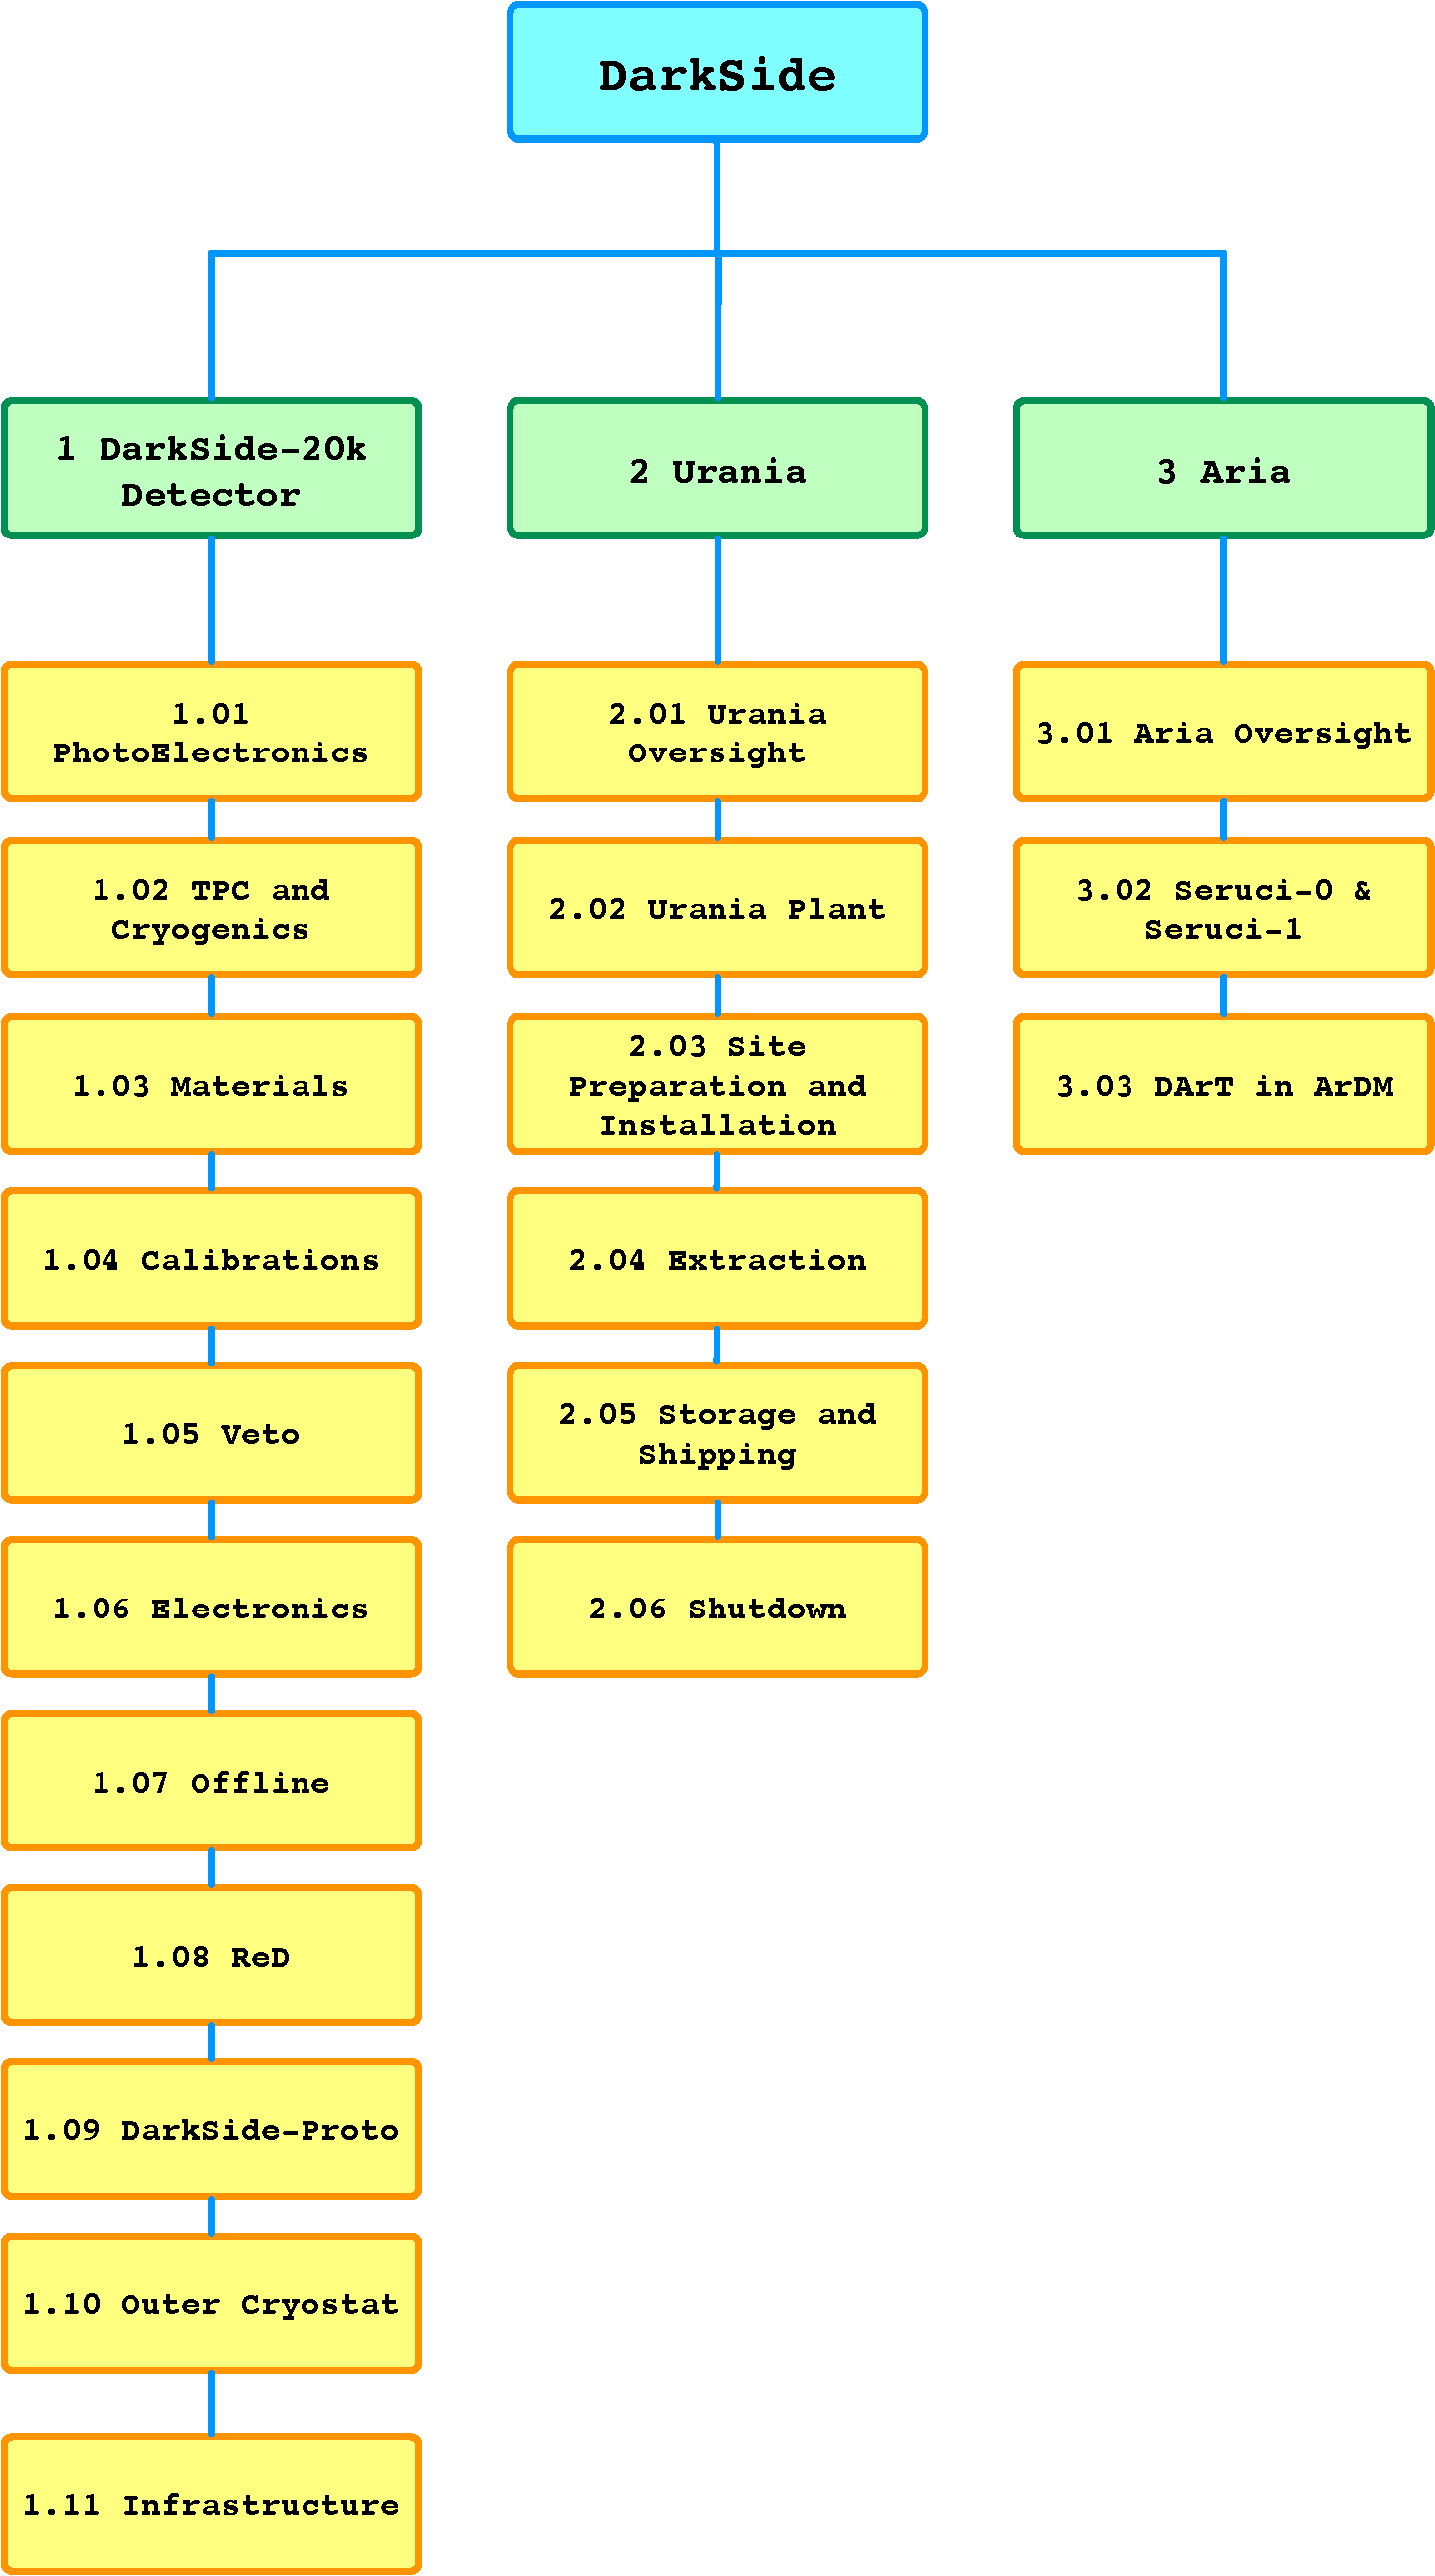
\includegraphics[height=\textheight]{./Figures/WBS.pdf}
\caption[Schematics of Work Breakdown Structure (\WBS)]{Schematics of the primary elements of the Work Breakdown Structure (\WBS), with details extending to Level~1.}
\label{fig:WBS} 
\end{figure} 


%---
\subsection{WBS Acronyms and Dictionary}

%---
\subsubsection{WBS acronyms}
\noindent {\bf \INFN} $\rightarrow$ Instituto Nazionale di Fisica Nucleare (Italy);\\
{\bf \NSF} $\rightarrow$ US National Science Foundation;\\
{\bf \NSF Mid-scale} $\rightarrow$ Specific \NSF\ funding solicitation which has been applied to;\\
{\bf \DOE} $\rightarrow$ US Department of Energy; \\
{\bf RAS} $\rightarrow$ funds from Regione Sardinia (Italy);\\
{\bf RA-CIPE} $\rightarrow$ funds from Regione Abtruzzo (Italy);\\
{\bf MIUR} $\rightarrow$ The Italian Ministry of Research and Education;\\
{\bf PREMIALE} $\rightarrow$ A special MIUR fund, reserved for a small number of selected projects;\\
{\bf CSN2} $\rightarrow$ The INFN Scientific Commission II, focusing on astrophysics and neutrino physics;\\
{\bf PON} $\rightarrow$ Programma Operativo Nazionale, a special MIUR fund, devoted to the infrastructure building;\\
{\bf MP} $\rightarrow$ Masterplan, a governament plan to develop the economy of the Regione Abruzzo;\\ 
{\bf PNNL LDRD} $\rightarrow$ PNNL Laboratory Directed Research \& Development;\\
{\bf STFC} $\rightarrow$ Science and Technology Facilities Counting, a UK organisation for Research and Innovation;\\ 
{\bf CFI} $\rightarrow$ Canadian Foundation for Innovation;\\
{\bf \IHEP} $\rightarrow$ Institute for High Energy Physics of the Chinese Academy of Science (China);\\
{\bf CNRS} $\rightarrow$ The French National Centre for Scientific Research;\\
{\bf IN2P3} $\rightarrow$ National Institute of Nuclear and Particle Physics;\\
{\bf AstroCeNT} $\rightarrow$ Astrophysics research centre in Poland;\\
{\bf UAr} $\rightarrow$ Underground Argon;\\
{\bf AAr} $\rightarrow$ Atmospheric Argon.\\


%---
\subsubsection{WBS Item description}
Table~\ref{tab:WBSTable} shows the WBS dictionary detailed to Level~1, with a brief description of the scope of each WBS item.

\begin{table}[t]
\centering
\resizebox{\textwidth}{!}{
\begin{tabular}{@{}p{1.2cm}@{}@{}p{6.7cm}@{}@{}p{12.5cm}@{} }
\hline
\hline
\multirow{1}{*}{{\bf \WBS}} 			&{\bf \WBS\ Name}						&{\bf \WBS\ Dictionary}\\
\hline\hline
\multirow{1}{*}{\bf 1} 					&{\bf \DSk\ Detector}					&\LArTPC\ and associated veto detector to be operated at \LNGS\ for \WIMP\ dark matter searches.\\
\hline
\multirow{1}{*}{1.01} 					&PhotoElectronics						&R\&D, fabrication, and testing of \DSkPdms\ low-background photosensors with photocathodic area of \DSkTilesArea, including procurement of \SiPMs, front end electronics, and optolink.\\
\hline
\multirow{1}{*}{1.02} 					&\TPC\ and Cryogenics					&Construction of \TPC, including \HV\ feedthrough and feed system, \PMMA\ vessel, coating with \TPB\ wavelength shifter, associated cryogenic purification and cooling loop, and \UAr\ storage and recovery systems.\\
\hline
\multirow{1}{*}{1.03} 					&Materials								&Material screening ad assay required to ensure achievement of overall background budget, including program of measurements with \ICPMS\ and \HPGe\ detectors and special \ce{Pb/Po} assay methods.\\
\hline
\multirow{1}{*}{1.04} 					&Calibrations							&Detector calibrations at large, including source deployment system, \grs, \AmC, \AmBe, \AmLi, and \ce{^252Cf} sources, and \UV\ \LEDs.\\
\hline
\multirow{1}{*}{1.05} 					&Veto									&Anti-coincidence \AAr-based veto detector, including \IAB, \GdAS, and \OAB\ instrumented with variant of the \LArTPC\ \DSkPdms.\\
\hline
\multirow{1}{*}{1.06} 					&Electronics							&Systems for \DAQ, trigger, and slow controls, including procurement of signal digitizers, VME crates, racks, development of \DAQ\ and slow controls software, and development of trigger architecture.\\
\hline
\multirow{1}{*}{1.07} 					&Offline								&\CPU\ and data storage, including development of overall computing model, data reconstruction frameworks and codes, data analysis frameworks and codes, and Monte-Carlo simulations.\\
\hline
\multirow{1}{*}{1.08} 					&\ReD									&Off-site, accelerator-based program of measurements for characterization of \LArTPCs\ response to \NRs\ and assessment of their possible directional response.\\
\hline
\multirow{1}{*}{1.09} 					&\DSp									&Development, construction, and operation at \CERN\ of the \DSpApproximateMass\ prototype required for a the characterization of the \DSks\ \LArTPC\ construction methods, photoelectronics, readout electronics, \DAQ\ and cryogenics.\\
\hline
\multirow{1}{*}{1.10} 					&Outer Cryostat							&Development, construction, and commissioning of the \pDUNE-like cryostat and associated cryogenics, and procurement of its \AAr\ fill.\\
\hline
\multirow{1}{*}{1.11} 					&Infrastructure							&Management of planning and installation of all necessary infrastructure items at \LNGS, including all safety analysis required for installation and operation.\\
\hline\hline
\multirow{1}{*}{\bf 2} 					&{\bf \Urania}							&Extraction, preliminary purification, and delivery of the \UraniaTotalDSkProduction\ \UAr\ batch required for the \DSk\ target.\\
\hline
\multirow{1}{*}{2.01} 					&\Urania\ Oversight						&Project management oversight of the \Urania\ sub-project installation, commissioning, and operation at the Kinder Morgan Doe Canyon Facility in Cortez, Colorado.\\
\hline
\multirow{1}{*}{2.02} 					&\Urania\ Plant							&Design and construction of a plant capable of extracting \UAr\ at a rate of \UraniaUArRate\ and chemical purity of \UraniaArFinalPurity, also including delivery at the Kinder Morgan Doe Canyon Facility in Cortez, Colorado.\\
\hline
\multirow{1}{*}{2.03} 					&Site Preparation and Installation		&Site preparation and development for the installation of the \Urania\ plant, including concrete work, electrical installation, feed optimization, procurement of control room and its installation, construction of buildings necessary to provide cover for the main equipment items, procurement of \UAr\ storage and shipping vessels, and development of truck loading and unloading areas.\\
\hline
\multirow{1}{*}{2.04} 					&Extraction								&Management oversight and labor required to perform the \UAr\ extraction, plant maintenance, and procurement of consumables ({\it i.e.}, electricity, \LIN, and other utilities).\\
\hline
\multirow{1}{*}{2.05} 					&Storage and Shipping					&Procurement of shipping and storage vessels for the \UraniaTotalDSkProduction\ \UAr\ batch, and shipping of said \UAr\ batch in said vessels from Cortez, Colorado, to Sardinia, Italy, and then from Sardinia to LNGS, Italy.\\
\hline
\multirow{1}{*}{2.06} 					&Shutdown								&Hand off of the \Urania\ site and plant to the next project assuming the lead for \UAr\ extraction at the Kinder Morgan Doe Canyon facility in Cortez, Colorado.\\
\hline\hline
\multirow{1}{*}{\bf 3} 					&{\bf \Aria}							&Chemical purification into detector grade argon of the the \UraniaTotalDSkProduction\ \UAr\ batch required for the \DSk\ target, verification of the \UAr\ purity with the \DArT\ detector at \LSC, study of isotopic separation capability of the \SeruciOne\ column, and its verification via the \DArT\ detector.\\
\hline
\multirow{1}{*}{3.01} 					&\Aria\ Oversight						&Project management oversight and installation, commissioning, and operation of the \Aria\ sub-project at the \Seruci, Sardinia, Italy site of the ''Monte Sinni'' mine operated by Carbosulcis, inclusive of labor and travel costs for the facility construction and labor and travel costs of regular staff of engineers and scientists for operation of the columns.\\
\hline
\multirow{1}{*}{3.02} 					&\SeruciZero\ and \SeruciOne\			&Procurement, construction, and installation of the \SeruciZero\ and \SeruciOne\ columns, including final dimensional verification and certification of leak rates first at the production site and then at \CERN, procurement and installation of the equipment and facilities items required for the operation of the columns, and labor costs required to assemble, train, and support the Operational Group for the columns run.\\
\hline
\multirow{1}{*}{3.03} 					&\DArT\ in \ArDM\						&Development, construction, installation, commissioning, and operation of the \DArT\ detector at \LSC, for the verification of the \ce{^39Ar} content of small argon batches processed with the \SeruciOne\ column.\\
\hline
\end{tabular}}
\caption[WBS Dictionary]{WBS Dictionary.}
\label{tab:WBSTable}
\end{table}


%---
\subsection{Scope Management Plan and Scope Contingency}
The scope of the project will be managed by the Project Scientists working in conjunction with the TB.  Changes in scope will be discussed within the TB as soon as the need for change is realized. The TB will receive the request for a change in scope, and after discussion with the Project Scientists, approve the change at a technical level or request a revised proposal for the change of scope. After technical approval, the change will go to the RRB who will confirm resources are available to accommodate the change.  Final approvals will be made by the supporting funding agency, following which, the change will go into effect.

Changes in scope must fall within the overall contingency of the project, which typically comes in the form of a \SI{20}{\percent}, built in contingency for major equipment and components and therefore should not result in an increase to the total project cost or to the cost of any single funding agency or partnering organization.  


%---
\subsection{Cost Estimating Plan, Cost Reports, and Baseline Budget}
Cost and schedule estimates are based on the WBS. The project has secured or anticipates funding from funding agencies across the globe operating in different currencies. Every item in the WBS clearly indicates the responsible funding agency and details the deliverable cost in the corresponding currency. Appendix~\ref{sec:AgencyView} presents the WBS organized by the activities assigned to each funding agency.

In addition, the funding agencies have been grouped into four different macro-areas, identified by the corresponding currency (USA (USD), Canada (CAN), Europe (EUR), and UK (GBP)). Each of these macro-areas is split into three columns (Labor Cost, Non-Labor Cost, and Total Cost), for a total of \num{12} columns in the \WBS. In addition, the global cost of the project, converted to USD where necessary, is shown in the three similar columns and identified by the name ``Global Cost'' (i.e. Global Labor Cost, Global Non-labor Cost, Global Total Cost).  The time schedule is reported in the form of a GANTT chart, also shown as part of the WBS tables in Appendix~\ref{sec:WBS} and Appendix~\ref{sec:AgencyView}.  


%---
\subsection{Budget contingency}
The \DSk\ project has identified cost, schedule, and contingency based on risks and uncertainties. Deliverable contingency is already included in the costs funded by INFN and NSF at a level of \SI{20}{\percent} for major equipment and components. Some of the WBS deliverables are not subject to contingency because the relevant contracts have already been executed and therefore costs are fixed and contingency could be safely removed. As an example, the contracts for the equipment items for SiPM packaging at \NOA\ (about \$4M) and the SiPM production by LFoundry (about \$6M) are already executed. The contingency on the packaging equipment items was removed. The contingency on unitary cost of SiPMs was also removed. The contingency on the required quantity of SiPMs remains at the appropriate \SI{20}{\percent} level. Other deliverable contingency mitigation strategies include realistic costs based on procurement offers and the selection of companies that in past interactions minimized the gap between the scheduled and the final cost. In addition, as a safety margin, the savings that will come from the competition among different companies submitting tender offers was not considered in the budget. It is worth noting that a large fraction of the budget has already been secured. A few potential triggers that would require the execution of a contingency plan have been identified. These are the possible loss of funding not yet secured, deliverable delays that impact personnel costs, and possible deliverable VAT increases.  The management of the budget contingency falls under the responsibility of the RRB.


%---
\subsection{Cost Book, Cost Model Data Set, and Basis of Estimate}
The Cost Book is stored within the Primavera P6 framework and is built from the bottom-up activity-based WBS.  The resulting output can be seen in Figure~\ref{fig:CostBook}, in a rolled-up form that shows the total project cost associated with each funding agency for both labor and non-labor elements of the project.  The full book, including all activities, is shown in Appendix~\ref{sec:AgencyView}.  The cost model data set comes from the L1 Managers after consultation with the L2 Managers and key responsible people within the Work Groups.  The data is maintained in an Excel spreadsheet and includes the hard-coded costs for each of the activities in the responsible institution's home currency.  This avoids complications due to fluctuating exchange rates and the corresponding issues that might arise in the P6 system.  This also allows for bookkeeping of activities in the currency that supports the effort. These can then be entered into the P6 system using global exchange rates to calculate the total project cost, either as a whole or on a per agency/institution basis, and presented in any of the four main currencies in use in the project. It is worth noting that Kinder Morgan provides UAr to Princeton University for free.

\begin{figure} [!th]
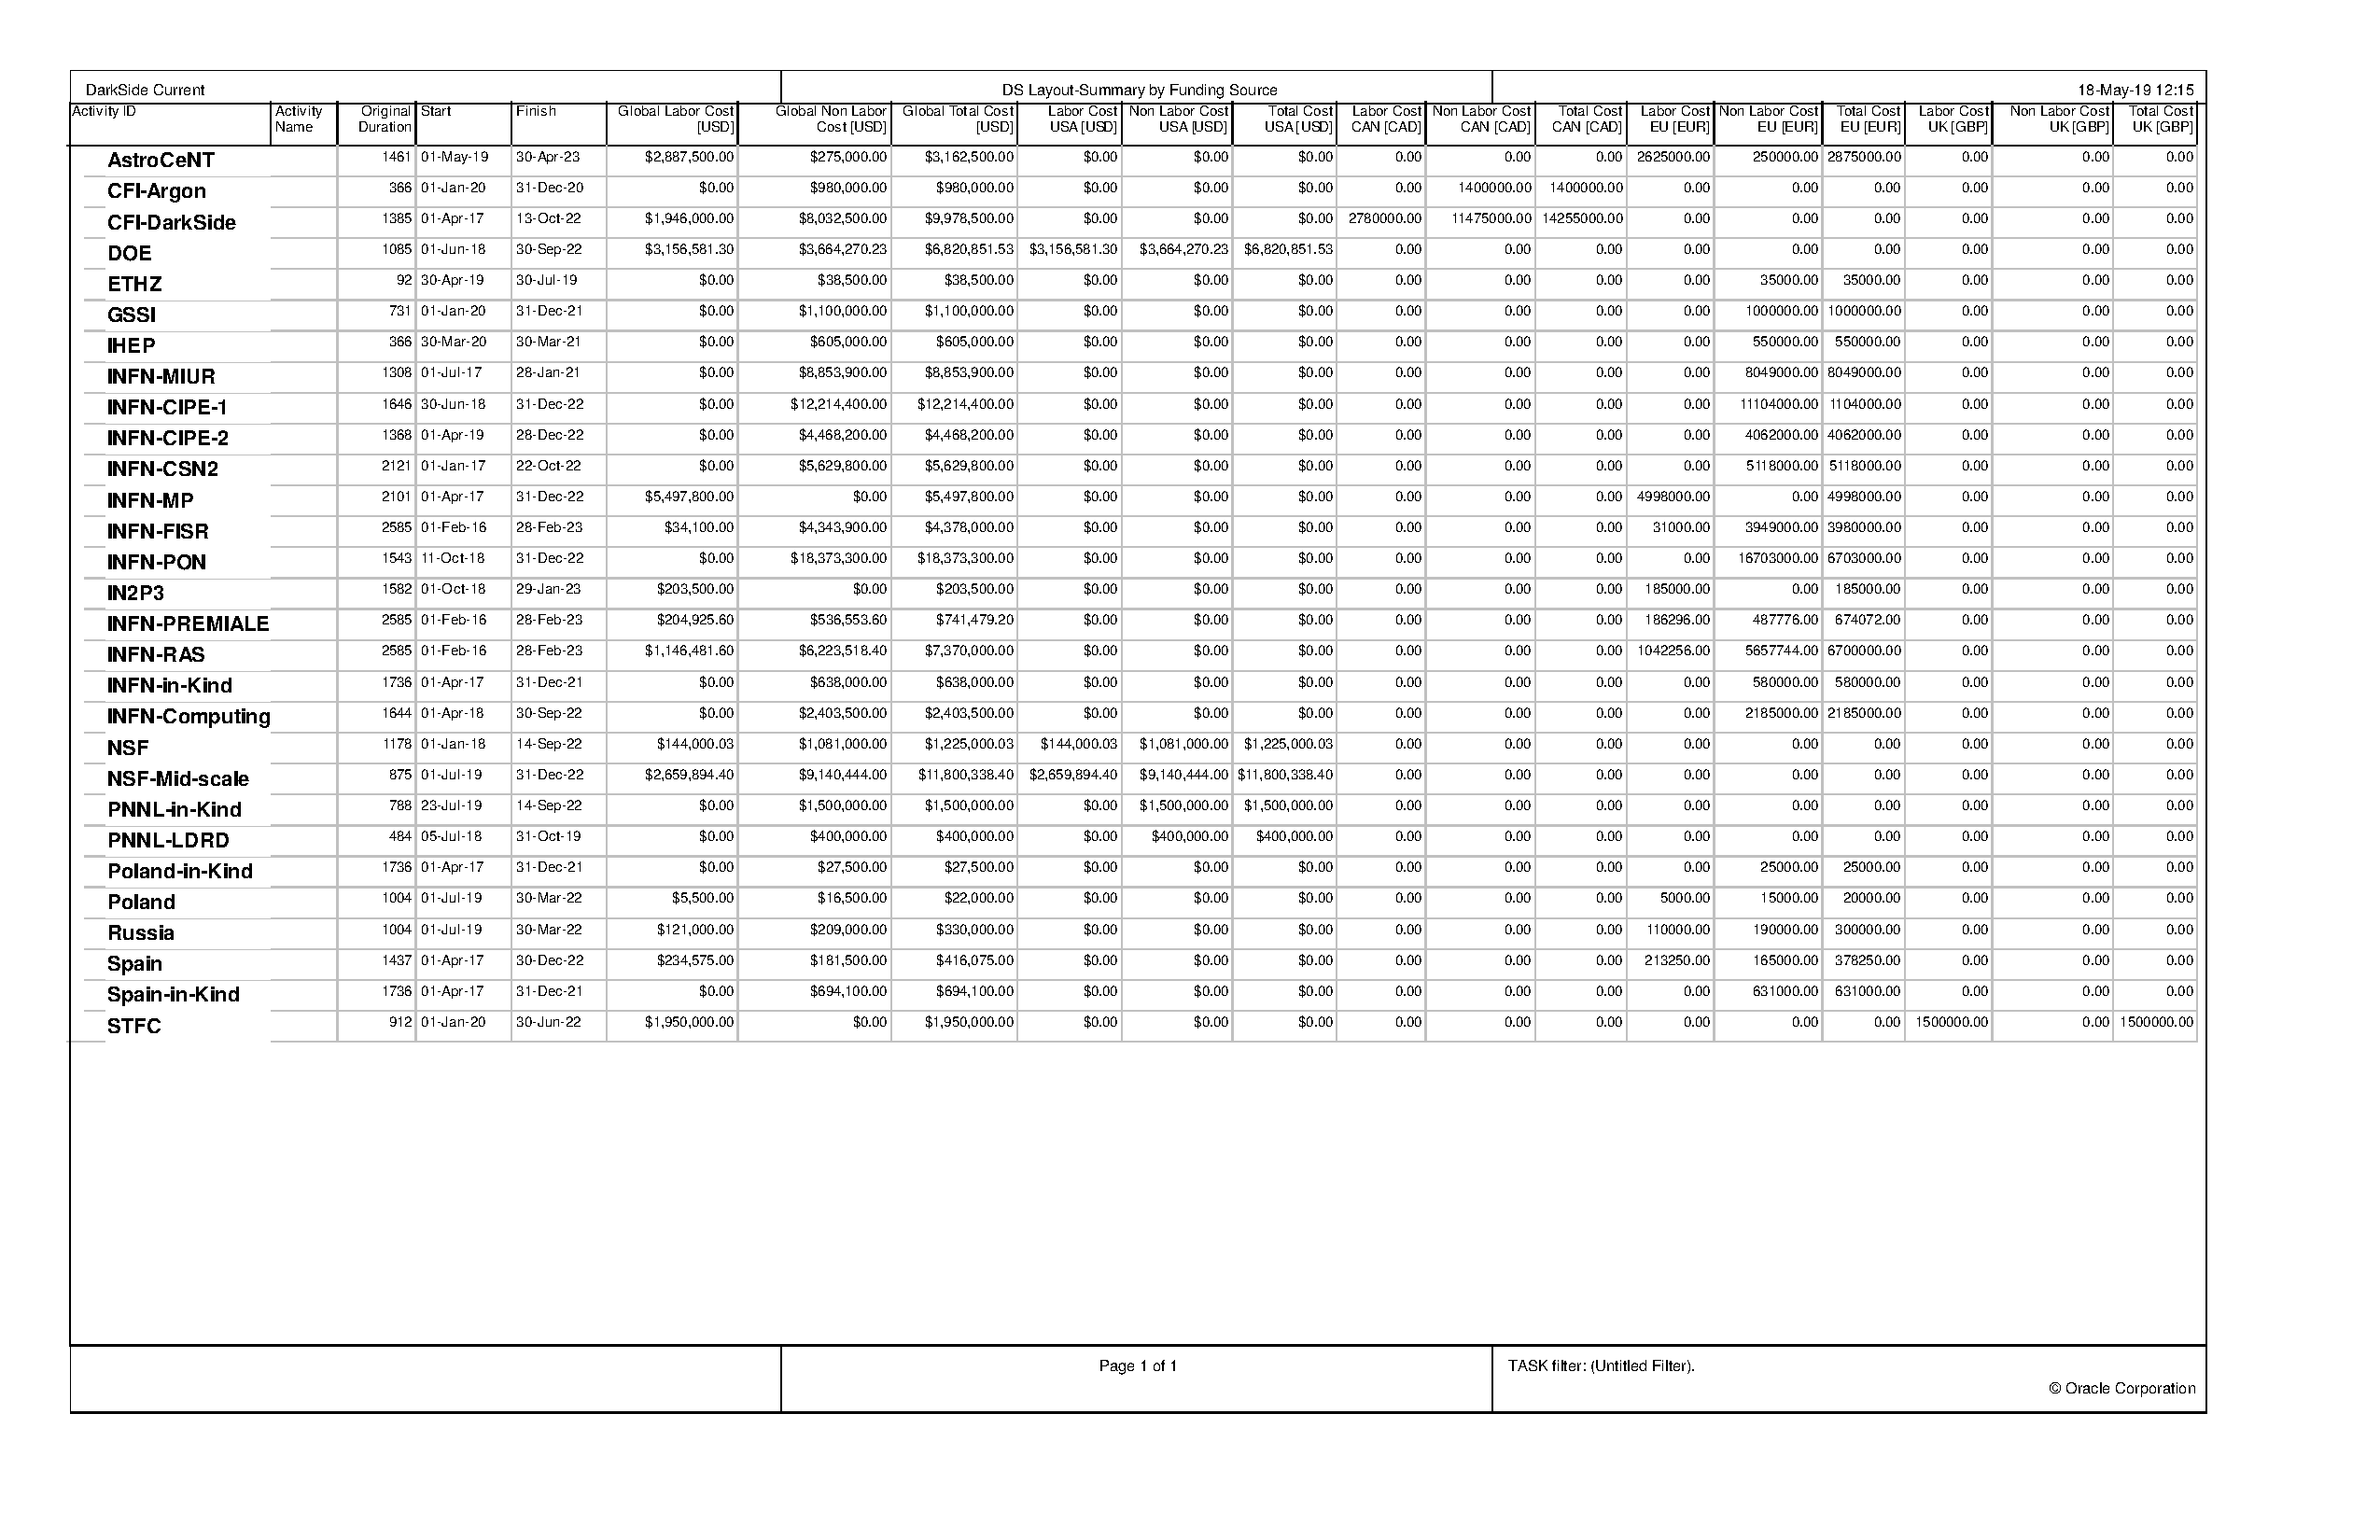
\includegraphics[rotate=90, width=0.85\columnwidth]{./Appendices/AgencyViewRolled.pdf}
\caption[Cost Book]{Cost Book rolled up by funding agency.}
\label{fig:CostBook} 
\end{figure} 

The project management team is working to obtain a proper Basis of Estimate for all major pieces of equipment using a bottom-up approach. This will continue until the project is defined down to single procurements or level of effort activities.  Some of the large and expensive components of the project have already had their procurement process started, and, in some cases, the tender for bidders to win the procurement or fabrication contract has been initiated.  For these items, the Basis of Estimate is quite well known and stems from quotes and or contracts that have been written for those specific items.  Other large pieces of equipment and components do not have a final design and therefore do not have official quotes. These have been estimated based on the prior experience of the Collaboration and/or on information from companies involved in the work.  For instance, many of the costs that have been assigned to the Urania site preparation and installation are proposals based on preliminary costs provided by contractors who will carry out the work; communications with vendors who will provide equipment, materials, and components; and the expert opinion of Kinder Morgan, which has experience in building industrial gas processing plants on the same site. This same methodology has been used for other parts of the project, although in some cases, when a main detector component is built from many smaller components, an engineering driven cost has been estimated based on the collaboration's experience in detector development, fabrication and installation, as well as quotes from vendors and local machine shops that carry out major fabrication work. The quotes for the most significant items planned to purchase with NSF funds are included as Supplementary Documents.

%---
\subsection{Funding Profile}

\begin{table}[t]
\begin{center}
\label{tab:FundingProfile}
\resizebox{\textwidth}{!}{
\begin{tabular}{l|r|r|r|r|r|r|r|r|r}
\hline
\hline
Funding Source	&\multicolumn{1}{c|}{FY2016}
							&\multicolumn{1}{c|}{FY2017}
										&\multicolumn{1}{c|}{FY2018}
													&\multicolumn{1}{c|}{FY2019}
																&\multicolumn{1}{c|}{FY2020}
																			&\multicolumn{1}{c|}{FY2021}
																						&\multicolumn{1}{c|}{FY2022}
																									&\multicolumn{1}{c|}{FY2023}
																												&\multicolumn{1}{c}{Total} \\
\hline
DOE				&			&    		&\$1,853	&\$7,647	&\$1,394,168&\$1,157,566&\$4,259,618&			&\$6,820,852\\
NSF 			&			&			&\$132,090	&\$472,713	&\$384,315	&\$73,332	&\$162,550	&			&\$1,225,000\\
NSF Mid-scale	&			&			&			&\$745,068	&\$4,867,707&\$4,588,856&\$1,554,922&\$43,786	&\$11,800,338\\
PNNL In-Kind	&			&			&			&\$22,321	&\$499,621	&\$501,282	&\$476,776	&			&\$1,500,000\\
PNNL LDRD		&			&			&\$72,727	&\$301,653	&\$25,620	&			&			&			&\$400,000\\
AstroCeNT		&			&			&			&\$302,387	&\$792,483	&\$927,255	&\$721,381	&\$418,994	&\$3,162,500\\
CFI-Argon		&			&			&			&			&\$733,661	&\$246,339	&			&			&\$980,000\\
CFI-DarkSide	&			&\$316,312	&\$636,199	&\$1,259,810&\$2,360,536&\$2,968,285&\$2,399,952&\$37,405	&\$9,978,500\\
ETHZ			&			&			&			&\$38,500	&			&			&			&			&\$38,500\\
GSSI			&			&			&			&			&\$412,312	&\$549,248	&\$138,440	&			&\$1,100,000\\
IHEP			&			&			&			&			&\$305,806	&\$299,194	&			&			&\$605,000\\
Poland-in-Kind	&			&\$2,899	&\$5,782	&\$5,782	&\$5,798	&\$5,782	&\$1,457	&			&\$27,500\\
Spain-in-Kind 	&			&\$72,009	&\$143,624	&\$143,648	&\$152,789	&\$145,829	&\$36,201	&			&\$694,100\\
INFN-in-Kind 	&			&\$15,074	&\$86,564	&\$468,568	&\$30,149	&\$30,066	&\$7,578	&			&\$638,000\\
IN2P3			&			&			&			&\$44,657	&\$49,278	&\$49,143	&\$46,119	&\$14,303	&\$203,500\\
INFN-CIPE-1		&			&			&\$138,654	&\$1,193,692&\$4,516,106&\$3,821,251&\$2,538,237&\$6,460	&\$12,214,400\\
INFN-CIPE-2		&			&			&			&\$234,768	&\$2,244,249&\$1,603,220&\$349,251	&\$36,713	&\$4,468,200\\
INFN-Computing	&			&			&\$267,543	&\$533,624	&\$535,086	&\$533,624	&\$533,624	&			&\$2,403,500\\
INFN-CSN2		&			&\$524,326	&\$868,166	&\$1,001,529&\$2,000,689&\$894,370	&\$292,319	&\$48,400	&\$5,629,800\\
INFN-FISR		&\$996,340	&\$1,508,057&\$1,508,057&\$348,817	&\$4,910	&\$4,896	&\$4,896	&\$2,026	&\$4,378,000\\
INFN-MIUR		&			&\$11,864	&\$47,069	&\$47,069	&\$6,252,294&\$2,495,604&			&			&\$8,853,900\\
INFN-MP			&			&\$16,814	&\$67,596	&\$312,706	&\$1,776,720&\$1,580,194&\$1,454,719&\$289,051	&\$5,497,800\\
INFN-PON		&			&			&			&\$2,007,013&\$8,834,101&\$5,412,501&\$1,928,362&\$191,323	&\$18,373,300\\
INFN-PREMIALE	&\$111,552	&\$167,557	&\$167,557	&\$98,014	&\$57,762	&\$57,604	&\$57,604	&\$23,831	&\$741,479\\
INFN-RAS		&\$323,557	&\$500,049	&\$513,503	&\$1,330,585&\$2,024,425&\$1,071,073&\$1,222,740&\$384,068	&\$7,370,000\\
Poland			&			&			&			&\$1,048	&\$14,970	&\$3,999	&\$1,983	&			&\$22,000\\
Russia			&			&			&			&\$30,239	&\$120,299	&\$119,970	&\$59,492	&			&\$330,000\\
Spain			&			&\$10,117	&\$23,974	&\$153,808	&\$104,428	&\$70,638	&\$44,284	&\$8,826	&\$416,075\\
STFC			&			&			&			&			&\$585,855	&\$780,428	&\$583,717	&			&\$1,950,000\\
\hline
Grand Total		&\$1,431,449&\$3,145,078&\$4,680,960&\$11,105,664
																&\$41,086,136
																			&\$29,991,549
																						&\$18,876,223
																									&\$1,505,184&\$111,822,244\\
\hline
\end{tabular}}
\caption[\DSk\ funding profile]{\DSk\ funding profile with breakdown by funding source and fiscal year.}
\end{center}
\end{table}

The funding profile is built from the \WBS, the resource driven schedule, and the negotiated division of responsibilities between collaborating institutions.  The expected funding profile for each of the US sources involved can be seen in Table~\ref{tab:FundingProfile}. The funding profile is deliverable-oriented and will be managed by the RRB.  The most important part of the funding profile is related to the construction of infrastructure required for deliverables, such as the \Urania\ and \Aria\ plants and the \NOA\ facility. Some deliverables, such as the \SiPM\ wafers, \num[group-separator={,}]{12000} channels of electronic digitizers, and many of the major detector components, are provided by companies or institutions selected through public tenders and already engaged through fixed terms contracts already executed.

Deliverables will be acquired using best-offer contracts based on detailed technical specifications.  Offers will be scored based on the provided technical specification and the cost.  The overall \DSk\ project execution will be managed by \INFN, in close communication with \NSF\ (and all peer funding agencies), and in accordance with the latest editions of relevant \INFN\ and \NSF\ manuals, guides and directives, industry codes and standards, and best practices in construction management.  Specific sub-deliverables under the exclusive responsibility of NSF (or other agency) will be managed in accordance with local manuals, guides, and directives.


%---
\subsection{Baseline Schedule Estimating Plan and Integrated Schedule}
The integrated schedule is built within the Primavera P6 system.  Each of the activities that are required for the success of the project have been included along with their expected duration time and their dependencies on other activities.  With these inputs, the logical ordering of the activities drives the baseline schedule, which has been produced and is shown in the right-most portion of the appropriate and relevant tables in the Appendices.  

%---
\subsection{Schedule Contingency}
The built-in schedule contingency for NSF and INFN is generally quantifiable as 20\%. This level of contingency has been added into the expected duration of the activities and sets a baseline for the overall contingency.  Many of the activities have been estimated in terms of the most conservative scenario possible within the schedule of the project.

In some specific cases, schedule contingency is dealt with directly. For example, the Urania tender includes a penalty that the contractor will incur if they miss the agreed upon delivery date. Other large tender items will follow a similar policy. It is worth noting that \SI{57}{\percent} of the funding for the project has been already secured, about \SI{4}{\percent} is partially secured, and just \SI{39}{\percent} is still being sought, of which, roughly \SI{30}{\percent} is for labor and \SI{70}{\percent} for non-labor.  In the case that the remaining labor funding were not secured, the most predictable consequence would be a delay of the project time schedule.  If the non-labor were not secured, an alternative plan would have to be implemented, for example sharing the unfunded costs between other funding agencies and/or involving new agencies.